% PHOTON: Live Photo Sync for Groups over Unreliable Mobile Networks
% Computer Networks (CSC-303) project report.
%
% Build: latexmk -pdf main.tex        (or ./build.sh in the parent folder, which also builds the Word report)
% Team details (group number, names, contacts, contributions) live in team.tex, generated from ../team.json.
\documentclass[11pt,a4paper]{article}

\usepackage[T1]{fontenc}
\usepackage[utf8]{inputenc}
\usepackage{mathptmx}                 % Times (Times New Roman metrics) for text and math
\renewcommand{\ttdefault}{lmtt}       % Latin Modern typewriter for code
\usepackage[margin=1in, headheight=22pt]{geometry}
\usepackage{amsmath,amssymb}
\usepackage{pifont}
\usepackage{graphicx}
\usepackage[table]{xcolor}
% Shared colours and TikZ styles. Used by main.tex and by figures/standalone.tex
% (which renders each figure to PNG for the Word report and the slides).
\usepackage{tikz}
\usetikzlibrary{arrows.meta,positioning,shapes.geometric,shapes.misc,fit,calc,backgrounds,shadows}
\usepackage{pgfplots}
\pgfplotsset{compat=1.18}

\definecolor{navy}{HTML}{1B365D}
\definecolor{pblue}{HTML}{2E6DB4}
\definecolor{headblue}{HTML}{2F5F98}
\definecolor{boxfill}{HTML}{EAF1FA}
\definecolor{boxline}{HTML}{6E9CD2}
\colorlet{blueline}{boxline}\colorlet{bluefill}{boxfill}
\definecolor{rowalt}{HTML}{EEF4FB}
\definecolor{redfill}{HTML}{FCEBEB}
\definecolor{redline}{HTML}{D9534F}
\definecolor{redtab}{HTML}{C62828}
\definecolor{greenfill}{HTML}{EAF6EA}
\definecolor{greenline}{HTML}{5CB85C}
\definecolor{greentab}{HTML}{2E7D32}
\definecolor{yellowfill}{HTML}{FFF6D5}
\definecolor{yellowline}{HTML}{D4A017}
\definecolor{orangefill}{HTML}{FDEBD8}
\definecolor{orangeline}{HTML}{E08A2E}
\definecolor{grayfill}{HTML}{EFEFEF}
\definecolor{grayline}{HTML}{8A8A8A}
\definecolor{purplefill}{HTML}{F1EAF8}
\definecolor{purpleline}{HTML}{8E6BBF}
\definecolor{codebg}{HTML}{F6F8FA}

\tikzset{
  >={Stealth[length=2.2mm]},
  every picture/.style={font=\small},
  blk/.style={draw=boxline, fill=boxfill, rounded corners=2pt, align=center, inner sep=4pt, minimum height=8mm, line width=0.6pt},
  svc/.style={blk, minimum width=26mm},
  cli/.style={blk, draw=greenline, fill=greenfill},
  ext/.style={blk, draw=grayline, fill=grayfill},
  bad/.style={blk, draw=redline, fill=redfill},
  warn/.style={blk, draw=yellowline, fill=yellowfill},
  edgeb/.style={blk, draw=orangeline, fill=orangefill},
  pur/.style={blk, draw=purpleline, fill=purplefill},
  store/.style={cylinder, shape border rotate=90, aspect=0.22, draw=greenline, fill=greenfill, align=center, minimum width=20mm, minimum height=11mm, inner sep=3pt, line width=0.6pt},
  arr/.style={->, draw=navy!80, line width=0.7pt},
  darr/.style={<->, draw=navy!80, line width=0.7pt},
  dsh/.style={->, draw=grayline, dashed, line width=0.7pt},
  hot/.style={->, draw=redtab, line width=1.1pt},
  lbl/.style={font=\scriptsize, fill=white, inner sep=1pt, align=center},
  lblc/.style={font=\scriptsize, inner sep=1pt, align=center},
  zone/.style={draw=grayline, dashed, rounded corners=4pt, inner sep=6pt},
  zonet/.style={font=\scriptsize\bfseries, text=grayline},
  st/.style={minimum width=22mm, minimum height=9mm},
  lifeline/.style={draw=grayline, dashed, line width=0.5pt},
  actor/.style={blk, minimum width=22mm, font=\small\bfseries},
  msg/.style={->, draw=navy!85, line width=0.6pt},
  rmsg/.style={->, draw=navy!60, dashed, line width=0.6pt},
}
                      % colours, TikZ styles and pgfplots (shared with the figure renderer)
\usepackage{array,tabularx,booktabs,colortbl}
\usepackage{enumitem}
\usepackage{float}
\usepackage[section]{placeins}        % floats stay inside their section
\usepackage[most]{tcolorbox}
\usepackage{listings}
\usepackage{fancyhdr}
\usepackage{titlesec}
\usepackage[font=small, labelsep=colon, skip=6pt]{caption}
\usepackage[hyphens,obeyspaces,spaces]{url}
\usepackage{needspace}
\usepackage{tocloft}
\renewcommand{\cftsecfont}{\bfseries\color{navy}}\renewcommand{\cftsecpagefont}{\bfseries}
\renewcommand{\cftsubsecfont}{\color{headblue}}
\setlength{\cftbeforesecskip}{5pt}\setlength{\cftbeforesubsecskip}{0.5pt}
\renewcommand{\cfttoctitlefont}{\color{headblue}\large\bfseries}
\setlength{\cftbeforetoctitleskip}{0pt}\setlength{\cftaftertoctitleskip}{8pt}
\renewcommand{\floatpagefraction}{0.75}\renewcommand{\topfraction}{0.85}\renewcommand{\bottomfraction}{0.6}\renewcommand{\textfraction}{0.12}
\usepackage[colorlinks=true, linkcolor=headblue, urlcolor=pblue, citecolor=headblue, pdfborder={0 0 0}]{hyperref}
\hypersetup{pdftitle={PHOTON: Live Photo Sync for Groups over Unreliable Mobile Networks}, pdfsubject={Computer Networks (CSC-303) project report}}

% Generated from team.json by tools/gen_team.py. Edit team.json and run ./build.sh,
% or edit this file directly if you only compile the LaTeX (for example on Overleaf).
\newcommand{\groupno}{13}
\newcommand{\institute}{Indian Institute of Technology Roorkee}
\newcommand{\instshort}{IIT Roorkee}
\newcommand{\department}{Department of Computer Science \& Engineering}
\newcommand{\course}{Computer Networks (CSC-303)}
\newcommand{\submittedto}{Prof. Sandeep Kumar}
\newcommand{\subdate}{3 November, 2026}
\newcommand{\versionline}{November 2026 $|$ Version 1.0}
\newcommand{\contacthead}{Email}
\newcommand{\memberrows}{%
  \relax Akshat Srivastava & 24114010 & \texttt{\footnotesize akshat\_s@cs.iitr.ac.in} & System design; Redis Functions library (sessions, announce, fencing, quota); orchestrator service \\
  \relax Shubham Singla & 24114093 & \texttt{\footnotesize shubham\_s@cs.iitr.ac.in} & Image server: resumable chunked upload with CRC32C, SHA-256 verification, sandboxed decoder, outbox \\
  \relax Yash Jain & 24114108 & \texttt{\footnotesize yash\_j2@cs.iitr.ac.in} & Network edge (Caddy, TLS 1.3, HTTP/3), WebSocket event plane, Redis Streams catch-up and resync \\
  \relax Pushkar Jain & 24114071 & \texttt{\footnotesize pushkar\_j@cs.iitr.ac.in} & Auth service: OAuth 2.0 with PKCE (Google, GitHub), EdDSA JWTs, refresh rotation; Redis ACLs \\
  \relax Aditya Yadav & 24114007 & \texttt{\footnotesize aditya\_y@cs.iitr.ac.in} & Android app (Kotlin): UI, MediaStore observer, foreground service, WorkManager upload, receive pipeline \\
  \relax Divyanshu Meena & 24114034 & \texttt{\footnotesize divyanshu\_m@cs.iitr.ac.in} & iOS PhotonKit, push (FCM/APNs), Docker deployment, tests and benchmarks, project report and slides \\
}


% ---------------------------------------------------------------- layout
\setlength{\parindent}{0pt}
\setlength{\parskip}{5pt plus 2pt}
\setlist{itemsep=2pt, topsep=3pt, parsep=1pt}
\renewcommand{\arraystretch}{1.2}
\setlength{\intextsep}{8pt plus 2pt minus 2pt}  % space around figures and tables placed with [H]
\setlength{\tabcolsep}{5pt}
\sloppy

\titleformat{\section}{\Needspace*{9\baselineskip}\color{headblue}\large\bfseries}{\thesection.}{0.5em}{}[{\color{headblue}\vspace{2pt}\titlerule[0.8pt]}]
\titleformat{\subsection}{\Needspace*{6\baselineskip}\color{headblue}\normalsize\bfseries}{\thesubsection}{0.7em}{}
\titleformat{\subsubsection}{\Needspace*{5\baselineskip}\color{headblue}\normalsize\bfseries\itshape}{\thesubsubsection}{0.7em}{}
\titlespacing*{\section}{0pt}{14pt}{8pt}
\titlespacing*{\subsection}{0pt}{10pt}{4pt}
\titlespacing*{\subsubsection}{0pt}{8pt}{3pt}
\setcounter{tocdepth}{2}

\pagestyle{fancy}
\fancyhf{}
\fancyhead[L]{\small\color{grayline}\instshort}
\fancyhead[C]{\small\color{headblue}\bfseries PHOTON}
\fancyhead[R]{\small\color{grayline}Group \groupno}
\fancyfoot[C]{\small\color{grayline}\thepage}
\renewcommand{\headrule}{\hbox to\headwidth{\color{headblue}\leaders\hrule height 0.6pt\hfill}}
\renewcommand{\footrule}{\hbox to\headwidth{\color{headblue}\leaders\hrule height 0.6pt\hfill}}
\renewcommand{\footrulewidth}{0.6pt}

% ---------------------------------------------------------------- tables
\newcommand{\hd}[1]{\textcolor{white}{\textbf{#1}}}            % header cell
\newcommand{\headrow}{\rowcolor{pblue}}                        % blue header row
\newcommand{\stripes}{\rowcolors{2}{white}{rowalt}}            % striped body rows
\newcolumntype{L}[1]{>{\raggedright\arraybackslash}p{#1}}
\newcolumntype{Y}{>{\raggedright\arraybackslash}X}
\newcolumntype{C}[1]{>{\centering\arraybackslash}p{#1}}
\newcommand{\cm}{\textcolor{greentab}{\ding{51}}}              % tick
\newcommand{\xm}{\textcolor{redtab}{\ding{55}}}                % cross
\newcommand{\pa}{\textcolor{orangeline}{Partial}}
\newcommand{\ep}[1]{\nolinkurl{#1}}                         % path or endpoint that may break at /
\arrayrulecolor{pblue}

% ---------------------------------------------------------------- boxes
% \begin{pbox}{blue|red|green|yellow}{Title} ... \end{pbox}
\colorlet{bluefill}{boxfill}\colorlet{blueline}{boxline}\colorlet{bluetab}{headblue}
\definecolor{yellowtab}{HTML}{9A7400}
\newtcolorbox{pbox}[2]{enhanced, breakable, colback=#1fill, colframe=#1line, boxrule=0.6pt, arc=2pt,
  left=6pt, right=6pt, top=8pt, bottom=5pt, fontupper=\small,
  attach boxed title to top left={xshift=4mm, yshift=-2.2mm},
  boxed title style={colback=#1tab, colframe=#1tab, arc=1.5pt, boxrule=0pt, top=1pt, bottom=1pt, left=5pt, right=5pt},
  coltitle=white, fonttitle=\small\bfseries, title={#2}, before skip=8pt, after skip=8pt}

% ---------------------------------------------------------------- code
\lstdefinestyle{code}{basicstyle=\ttfamily\footnotesize, backgroundcolor=\color{codebg}, frame=single, rulecolor=\color{boxline},
  framesep=4pt, xleftmargin=6pt, xrightmargin=6pt, columns=fullflexible, keepspaces=true, breaklines=true,
  showstringspaces=false, commentstyle=\color{grayline}\itshape, keywordstyle=\color{headblue}\bfseries, aboveskip=6pt, belowskip=6pt}
\lstset{style=code}

% ---------------------------------------------------------------- figures and screenshots
\newcommand{\fig}[1]{\input{figures/#1}}
% \appshot{file}{label text}: an app screenshot if screens/<file> exists, otherwise a placeholder frame.
\newcommand{\appshot}[2]{%
  \IfFileExists{screens/#1}{\includegraphics[height=7cm, keepaspectratio]{screens/#1}}{%
  \begin{tikzpicture}
    \draw[grayline, fill=grayfill, rounded corners=10pt, line width=1pt] (0,0) rectangle (3.4,7);
    \draw[grayline, rounded corners=2pt] (1.2,6.7) rectangle (2.2,6.82);
    \node[align=center, font=\scriptsize, text width=3.0cm, text=grayline] at (1.7,3.5) {\textbf{#2}\\[4pt]screenshot to add:\\\texttt{\tiny report/screens/\\#1}\\[4pt]\texttt{\tiny adb exec-out\\screencap -p > #1}};
  \end{tikzpicture}}}

\begin{document}

% BEGIN-TITLEPAGE (the Word report builds its own title page from team.json)
\newgeometry{top=0.75in, bottom=0.7in, left=1in, right=1in}
\begin{titlepage}
\thispagestyle{empty}
\centering

\includegraphics[width=2.5cm]{images/iitr-logo.png}\par\vspace{5mm}
\begin{tcolorbox}[colback=navy, colframe=navy, arc=3pt, boxrule=0pt, halign=center, top=7pt, bottom=7pt, width=\linewidth]
  {\color{white}\large\bfseries \institute\par}\vspace{3pt}
  {\color{white!88!navy}\small \department\par}\vspace{2pt}
  {\color{white!88!navy}\small Subject: \course\ \ $|$\ \ Project Report\par}
\end{tcolorbox}
\vspace{4mm}
{\color{headblue}\rule{\linewidth}{0.6pt}}\par\vspace{3mm}
{\color{navy}\fontsize{30}{34}\selectfont\bfseries PHOTON\par}\vspace{2mm}
{\color{headblue}\large\bfseries Live Photo Sync for Groups over Unreliable Mobile Networks\par}\vspace{3mm}
{\color{grayline}\itshape A verified, resumable and ephemeral photo-sharing system\\built on HTTP/3, WebSocket and Redis Streams\par}
\vspace{3mm}{\color{headblue}\rule{\linewidth}{0.6pt}}\par\vspace{3mm}
{\color{navy}\Large\bfseries Group No. \groupno\par}\vspace{2mm}
{\color{grayline}\textbf{Submitted To:} \submittedto\par}\vspace{1mm}
{\color{grayline}\textbf{Submission Date:} \subdate\par}
\vspace{4mm}
\begin{tcolorbox}[enhanced, colback=boxfill, colframe=boxline, boxrule=0.6pt, arc=2pt, left=4pt, right=4pt, top=8pt, bottom=4pt,
  attach boxed title to top left={xshift=4mm, yshift=-2.2mm}, boxed title style={colback=headblue, colframe=headblue, arc=1.5pt, boxrule=0pt},
  coltitle=white, fonttitle=\small\bfseries, title={Group Members \& Contributions}]
\footnotesize\rowcolors{2}{white}{rowalt}
\begin{tabularx}{\linewidth}{L{2.35cm}L{1.55cm}L{4.15cm}Y}
\headrow \hd{Name} & \hd{Enroll. No.} & \hd{\contacthead} & \hd{Individual Contribution}\\
\memberrows
\end{tabularx}
\end{tcolorbox}
\vfill
{\color{headblue}\rule{\linewidth}{0.6pt}}\par\vspace{2mm}
{\color{grayline}\small \versionline\par}
\end{titlepage}
\restoregeometry
% END-TITLEPAGE

% BEGIN-TOC
\pagenumbering{arabic}
\setcounter{page}{1}
{\hypersetup{linkcolor=headblue}\tableofcontents}\thispagestyle{fancy}
\clearpage
% END-TOC

\section{Introduction}\label{sec:intro}

\subsection{Background}

A group of people at a wedding, a field trip or a hackathon takes hundreds of photos, and every photo ends up on the one phone that took it. Getting the photos to everyone else is still a manual job: someone creates a shared album days later, people forward pictures one by one in a chat, or the group gives up. The photos exist; the network between the phones is what is missing.

PHOTON closes that gap. Members join a live \emph{session} with a short code or a QR code, and from then on every photo any member takes appears in every other member's gallery, without anyone pressing a button. The server keeps a photo only for 30 minutes, long enough for the group's phones to fetch it.

Behind this simple behaviour sit most of the topics of a computer networks course:

\begin{itemize}
  \item \textbf{Application-layer protocols.} The system uses HTTP/1.1, HTTP/2 and HTTP/3 for requests and bulk transfer, WebSocket for a long-lived event channel, and push services (FCM, APNs) as wake-up signals.
  \item \textbf{Transport protocols.} TCP carries the control and event planes; QUIC over UDP carries photo data, because it survives a phone moving from Wi-Fi to cellular and it does not stall every stream when one packet is lost.
  \item \textbf{Reliable delivery over an unreliable network.} Large uploads are cut into checksummed chunks, sent several at a time, and only the missing chunks are resent, which is selective repeat at the application layer. Every request is idempotent, so a retry after a timeout is always safe.
  \item \textbf{Publish/subscribe with a durable log.} Events go into a Redis Stream and are read by one loop per client, so a client that reconnects receives exactly what it missed.
  \item \textbf{Network security.} TLS 1.3 protects every hop. Users sign in with OAuth 2.0 and PKCE and receive signed JSON Web Tokens. Photos are content-addressed by SHA-256, and the server recomputes the hash itself instead of trusting the client.
  \item \textbf{Distributed state.} Sessions and photo status live in Redis and change only through atomic server-side scripts. Late messages from a slow client are rejected with \emph{fencing tokens}, so they can never undo newer state.
\end{itemize}

\subsection{Motivation}

Four concrete problems drove the design of PHOTON.

\begin{enumerate}
  \item \textbf{Sharing is manual and late.} Shared albums and chat groups need someone to pick photos and send them. By the time that happens the event is over, and many photos are never shared.
  \item \textbf{Cloud albums keep everything, forever.} Existing services store every shared photo indefinitely, tie the group to one vendor's ecosystem, or recompress the images. A group that only wants to exchange photos during an event should not leave a permanent copy on someone else's server.
  \item \textbf{Mobile networks are hostile to large uploads.} A 4\,MB photo uploaded over a single HTTP request restarts from zero when the phone changes network, a lift cuts the signal or the operating system suspends the app. Retries that are not idempotent create duplicates, and notifications that are lost leave members with gaps.
  \item \textbf{A client's claim is not proof.} If the server trusts the hash a client announces, one member can upload different bytes under the hash of someone else's real photo, and deduplication then hides the real photo from everyone. The server has to verify the bytes before telling anyone the photo exists.
\end{enumerate}

\subsection{Application Domain}

\begin{pbox}{blue}{Where PHOTON Is Used}
\textbf{1. Events and trips:} weddings, college fests, family trips and sports days, where many people photograph the same moments and everyone wants everyone's photos.\par\smallskip
\textbf{2. Education and teams:} field labs, site visits and hackathons, where a team documents its work on several phones and needs one shared record during the activity.\par\smallskip
\textbf{3. Inspections and incident reporting:} surveyors, insurance assessors or volunteers who must get photos from the field to their colleagues at once, without keeping them on a third-party cloud afterwards.\par\smallskip
\textbf{4. Any short-lived group:} a session lasts hours, not years, and server copies are deleted 30 minutes after they are stored, so nothing outlives the event on the server.
\end{pbox}

\subsection{Problem Statement}

\begin{pbox}{red}{Core Problem Statement}
How can a group of phones, connected through unreliable and changing mobile networks, share every photo taken during a live session with every other member automatically, so that each photo is uploaded once, verified before anyone is told about it, delivered to every member without gaps or duplicates even across disconnections, and removed from the server within a bounded time?
\end{pbox}

\subsection{Objectives and Scope}

The objectives of the project were to:

\begin{enumerate}
  \item detect a new camera photo on the device and sync it while the user is in a session, also while the app is in the background;
  \item upload each photo once per session, using its SHA-256 hash as the content address;
  \item show a thumbnail first, then a preview, then save the original, according to network conditions;
  \item announce a photo to the group only after the server has verified its hash and stored it;
  \item deliver every event to every member at least once and in order, with deduplication on the client so that each photo is processed exactly once;
  \item make a photo unavailable exactly 30 minutes after it is stored and delete the file within 5 minutes after that;
  \item protect every hop with TLS 1.3 and every request with a verified identity.
\end{enumerate}

Out of scope for this version are video and Live Photos, photos taken before joining, long-term backup, more than one active session per user, and a web client (a browser cannot watch the phone's gallery).

\section{Networking Background and Design Rationale}\label{sec:background}

This chapter introduces the networking concepts PHOTON is built on and explains, for each kind of traffic, why one protocol was chosen over the alternatives.

\subsection{Networking Concepts Used in PHOTON}

Table~\ref{tab:concepts} maps each concept to the standard that defines it and to the place where PHOTON uses it.

\begin{table}[H]
\centering
\small\stripes
\begin{tabularx}{\linewidth}{L{3.4cm}L{2.9cm}Y}
\headrow \hd{Concept} & \hd{Standard} & \hd{Role in PHOTON}\\
HTTP semantics, status codes, idempotent methods & RFC 9110 & Every REST call; the error contract maps each failure to a status code and a retry rule; chunk \texttt{PUT}s are idempotent \\
HTTP/2 multiplexing & RFC 9113 & Several chunk uploads share one TCP connection; fallback when UDP is blocked \\
QUIC and HTTP/3 & RFC 9000, 9114 & Data plane over UDP 443: no head-of-line blocking between streams, 1-RTT setup, connection migration across networks \\
Alternative services (Alt-Svc) & RFC 7838 & The edge advertises \texttt{h3} on UDP 443; clients switch to it and fall back to HTTP/2 automatically \\
TLS 1.3 & RFC 8446 & Every hop, including service-to-service calls and Redis \\
WebSocket & RFC 6455 & Full-duplex event channel; binary protobuf frames; application close codes 4001--4410 \\
OAuth 2.0 with PKCE & RFC 6749, 7636 & Sign-in through Google or GitHub without a client secret on the phone \\
JSON Web Token, EdDSA & RFC 7519, 8037 & Access tokens and per-photo upload tokens, verified locally by each service \\
CRC32C, SHA-256 & RFC 3720, FIPS 180-4 & Per-chunk integrity check; content address and end-to-end verification of each photo \\
Reverse proxy, forwarded client address & RFC 7239 & Caddy terminates TLS; \texttt{X-Forwarded-For} is trusted only from known proxies, for per-IP rate limits \\
Publish/subscribe over a durable log & Redis Streams & Gap-free event delivery with a resumable cursor \\
Push notifications & FCM, APNs & Best-effort wake-up hint for phones without an open socket \\
Port forwarding & Android \texttt{adb reverse} & A phone on USB reaches the laptop's development server through a tunnel \\
\end{tabularx}
\caption{Networking concepts, their standards, and their role in PHOTON}\label{tab:concepts}
\end{table}

\subsection{Choosing a Protocol for Each Plane}

PHOTON separates its traffic into four planes, because each has different needs: small requests that must be answered, events that must reach the phone as soon as they happen, megabytes of photo data that must survive bad networks, and calls between services that must be authenticated. Table~\ref{tab:planes} lists the options considered for each plane.

\begin{table}[H]
\centering
\small\stripes
\begin{tabularx}{\linewidth}{L{2.2cm}L{3.9cm}L{3.1cm}Y}
\headrow \hd{Plane} & \hd{Options considered} & \hd{Chosen} & \hd{Reason}\\
Control (client to orchestrator) & Raw TCP protocol, gRPC, HTTP with JSON, HTTP with protobuf & HTTPS with protobuf bodies (\ep{application/x-protobuf}) & FastAPI serves HTTP, not raw sockets; status codes, headers, proxies and retries come for free; protobuf keeps bodies small \\
Events (orchestrator to client) & Polling, long polling, Server-Sent Events, push only, WebSocket & WebSocket, plus FCM/APNs as a hint & One open socket delivers an event within a few milliseconds; push alone may be dropped, delayed or merged, so it only wakes the app \\
Data (client and image server) & One large HTTP/1.1 \texttt{PUT}, raw TCP, HTTP/2, HTTP/3 & HTTP/3 over QUIC, HTTP/2 fallback, chunked and resumable & QUIC survives network changes and avoids head-of-line blocking; chunks bound the cost of a failure to 1\,MiB \\
Internal (service to service) & Shared database writes, message queue, HTTPS & HTTPS with a service JWT (mTLS optional) & Only the image server may report a photo as stored; every report is authenticated and fenced \\
\end{tabularx}
\caption{Protocol options considered for each plane}\label{tab:planes}
\end{table}

\paragraph{Why not a hand-built TCP protocol?} An early version of the design used raw TCP between the phone and the server and a hand-written fallback from QUIC to TCP. Both were dropped. HTTP already defines request framing, status codes, authentication headers and caching rules, and every proxy, load balancer and monitoring tool understands it. Standard HTTP/3 clients (Cronet on Android, \texttt{URLSession} on iOS) already fall back to HTTP/2 when UDP is blocked. A custom protocol would have repeated all of this with more bugs.

\paragraph{Why QUIC for photo data?} Over TCP, one lost segment stalls every HTTP/2 stream on the connection until it is retransmitted, so a lost packet in chunk 2 also delays chunks 3 and 4. QUIC delivers each stream independently. QUIC also identifies a connection by a connection ID rather than by the address and port pair, so when a phone moves from Wi-Fi to LTE its new address can continue the same connection, where TCP would have to start again with a new handshake.

\subsection{Protocol Stack}

Figure~\ref{fig:stack} shows the protocol stack of each plane. All planes share the same payload format (protobuf) and the same network layer; they differ in the application and transport protocols.

\begin{figure}[H]
\centering
\resizebox{0.95\linewidth}{!}{\fig{stack}}
\caption{Protocol stack of the four planes}\label{fig:stack}
\end{figure}

\subsection{Reliability Concepts}

Four ideas from networking and distributed systems recur throughout the design.

\begin{enumerate}
  \item \textbf{At-least-once delivery plus idempotency gives an exactly-once effect.} The network may duplicate or drop messages, so the sender retries and the receiver makes a repeat harmless. PHOTON's chunk uploads, \texttt{complete} calls, reports and event deliveries are all built this way.
  \item \textbf{Selective repeat.} As in the sliding-window protocols of the transport layer, the receiver tells the sender exactly which pieces arrived, and only the missing ones are sent again (Section~\ref{sec:alg-upload}).
  \item \textbf{Leases.} A reservation that is not renewed expires on its own, so a client that disappears cannot hold a resource forever. Each upload holds a 15-minute lease that every chunk renews.
  \item \textbf{Fencing tokens.} Every message that changes upload state names the \texttt{upload\_id} it belongs to, and the server applies it only if that id is still the live one, so a delayed message from an old attempt is rejected.
\end{enumerate}

Retries use exponential backoff with jitter, so that phones which lost the network together do not all retry at the same instant. The delay before attempt $k$ is
\begin{equation}\label{eq:backoff}
  d_k = \tfrac{1}{2}s_k + U\!\left(0,\ \tfrac{1}{2}s_k\right), \qquad s_k = \min\!\left(60\ \text{s},\ 1\ \text{s}\cdot 2^{k}\right),
\end{equation}
where $U(a,b)$ is a uniformly random value. A \texttt{Retry-After} from the server, when present, replaces $d_k$.

\section{Proposed System}\label{sec:proposed}

\subsection{Overview}

PHOTON is a client--server system with three server services, three data stores and native mobile clients. One rule shapes the whole design:

\begin{pbox}{blue}{Design Rule}
A photo is announced to the session only after the image server has recomputed its SHA-256 over the received bytes, found it equal to the hash the uploader claimed, and stored the file. Until then the photo does not exist for anyone else.
\end{pbox}

Each kind of state has exactly one writer. The \textbf{orchestrator} owns sessions, members, photo status and event fan-out, and never touches image bytes. The \textbf{image server} owns the bytes, thumbnails, previews and deletion, and never changes session state or talks to members; it only reports to the orchestrator. The \textbf{Auth} service owns the signing key and issues tokens, but is not in the path of every request, because the other services verify tokens locally with its public key. The \textbf{client} owns the gallery observer, the upload queue and its local record of received photos, but never decides on its own what counts as a duplicate.

\subsection{System Architecture Block Diagram}

Figure~\ref{fig:arch} shows the components and the protocols between them. All client traffic enters through one edge proxy, which terminates TLS 1.3 and offers HTTP/3 on UDP port 443 next to HTTP/2 on TCP port 443. The highlighted arrow is the only path by which a photo becomes visible: the image server's fenced report to the orchestrator.

\begin{figure}[H]
\centering
\resizebox{\linewidth}{!}{\fig{arch}}
\caption{System architecture block diagram}\label{fig:arch}
\end{figure}


\subsection{Steps of the Proposed System}\label{sec:steps}

\begin{enumerate}[label=\textbf{Step \arabic*:}, leftmargin=*, align=left]
  \item \textbf{Sign in.} The app signs in with Google (native ID token) or GitHub (browser, Authorization Code with PKCE) and receives a 15-minute access JWT and a rotating refresh token.
  \item \textbf{Create or join.} The host creates a session and gets an 8-character code, an invite link and a QR code. Members join with any of them. One Lua script checks that the session is \texttt{ACTIVE}, not full, and that the user has no other live session.
  \item \textbf{Connect.} The app opens the WebSocket \texttt{/v1/ws}, authenticates in the first frame, loads the snapshot and resumes the event stream from its cursor. It starts a foreground service that watches the gallery.
  \item \textbf{Detect.} When the camera saves a photo, the observer records it in a local queue. A WorkManager job computes its SHA-256 and removes GPS data from a copy.
  \item \textbf{Announce.} The app sends the hash and size. The orchestrator answers \texttt{UPLOAD} (with an upload token), \texttt{ALREADY\_UPLOADED} or \texttt{IN\_PROGRESS}.
  \item \textbf{Upload.} The app sends 1\,MiB chunks, three at a time, each with a CRC32C, then calls \texttt{complete}. After a failure it asks which chunks arrived and sends only the rest.
  \item \textbf{Verify.} The image server assembles the file, recomputes SHA-256, validates and decodes it in a sandboxed process, makes a thumbnail, and writes the metadata with \texttt{expires\_at = stored\_at + 30 min}.
  \item \textbf{Report and announce.} The image server reports \texttt{stored} with the \texttt{upload\_id}. If the id is still the live one, the orchestrator marks the photo \texttt{STORED} and appends \texttt{PHOTO\_STORED} to the session's stream in the same script.
  \item \textbf{Deliver.} Every member's WebSocket loop reads the new event and sends it; members without a socket get a push hint and catch up when they wake.
  \item \textbf{Receive.} Each member fetches the thumbnail, then the preview, then the original, each with its own JWT, and saves only the original to the gallery.
  \item \textbf{Expire, recall or end.} At \texttt{expires\_at} every download is refused and the file is deleted within 5 minutes. The uploader or host can recall a photo earlier, and the host can end the session, which deletes everything.
\end{enumerate}

\subsection{Life of a Photo}

Figure~\ref{fig:seq} follows one photo through the system as a sequence diagram. Messages 1--3 are the control plane, 4--7 the data plane, 8--10 the internal plane, and 12--14 the event and data planes on the receiving side.

\begin{figure}[H]
\centering
\resizebox{0.92\linewidth}{!}{\fig{seq}}
\caption{Life of a photo: from announce to every member's gallery}\label{fig:seq}
\end{figure}

\subsection{Wire Protocol and API}

\subsubsection{Endpoints}

\begin{table}[H]
\centering
\small\stripes
\begin{tabularx}{\linewidth}{L{6.4cm}L{1.9cm}Y}
\headrow \hd{Endpoint} & \hd{Caller} & \hd{Purpose}\\
\ep{POST /v1/auth/oauth/start}, \ep{/callback} & client & Browser sign-in with \texttt{state} and PKCE \\
\ep{POST /v1/sessions}, \ep{/v1/sessions/join} & client & Create (code, invite link, QR), join by code or invite \\
\ep{GET /v1/sessions/{sid}/snapshot} & client & Members, live photos, recalled hashes and a cursor \\
\ep{WS /v1/ws} & client & Live events; first frame is \texttt{Hello} \\
\ep{POST /v1/photos/announce} & client & \texttt{UPLOAD}, \texttt{ALREADY\_UPLOADED} or \texttt{IN\_PROGRESS} \\
\ep{PUT /v1/uploads/{id}/chunks/{n}} & client & One chunk, with \texttt{X-Chunk-CRC32C} \\
\ep{GET /v1/uploads/{id}} & client & Which chunks arrived, so an upload can resume \\
\ep{POST /v1/uploads/{id}/complete} & client & Idempotent: 202 while verifying, then always the same result \\
\ep{GET /v1/sessions/{sid}/photos/{hash}?size=} & client & \texttt{thumb}, \texttt{preview} or \texttt{full}; checked on every request \\
\ep{POST /internal/v1/photos/stored}, \ep{/rejected} & image server & Fenced report carrying the \texttt{upload\_id} \\
\ep{DELETE /internal/v1/photos/{sid}/{hash}} & orchestrator & Delete after expiry, recall or end; retried until acknowledged \\
\end{tabularx}
\caption{Main endpoints (all bodies are protobuf)}\label{tab:endpoints}
\end{table}

\subsubsection{Messages}

All messages are defined once in \texttt{proto/photon.proto} and shared by the Python services, the Kotlin app and the Swift library. Field numbers are never reused, so old and new clients can talk to the same server. The core messages are:

\begin{lstlisting}[language=C]
message AnnounceRequest {
  bytes sha256 = 1;  uint64 size = 2;  string mime = 3;
  int64 taken_at_ms = 4;  string session_id = 5;
}
message AnnounceResponse {
  enum Result { UPLOAD = 0; ALREADY_UPLOADED = 1; IN_PROGRESS = 2; }
  Result result = 1;  string upload_id = 2;  string upload_url = 3;
  string upload_token = 4;  uint32 chunk_size_hint = 5;
}
message PhotoEvent {
  enum Type { PHOTO_STORED = 0; PHOTO_RECALLED = 1; MEMBER_JOINED = 2;
              MEMBER_LEFT = 3; SESSION_ENDED = 4; HOST_CHANGED = 5; }
  string event_id = 1;  Type type = 2;  string session_id = 3;  bytes sha256 = 4;
  string uploader_id = 5;  uint64 size = 6;  int64 taken_at_ms = 7;
  int64 expires_at_ms = 8;  string member_id = 9;
}
message Error {
  string code = 1;  string message = 2;  bool retryable = 3;
  uint32 retry_after_s = 4;  repeated uint32 missing_chunks = 5;
}
\end{lstlisting}

A \texttt{PhotoEvent} carries no download link. Receivers fetch by hash with their own JWT, so a leaked event is useless on its own.

\subsubsection{Error Contract}

Every error has one status code, one machine-readable code and one client action (Table~\ref{tab:errors}). The client retries only when \texttt{retryable} is true and waits \texttt{retry\_after\_s} when it is set.

\begin{table}[H]
\centering
\small\stripes
\begin{tabularx}{\linewidth}{C{1.0cm}L{6.2cm}Y}
\headrow \hd{Status} & \hd{Codes} & \hd{Client action}\\
400 & \texttt{INVALID\_REQUEST} (lists missing chunks) & Fix the request; send the missing chunks \\
401 & \texttt{TOKEN\_EXPIRED}, \texttt{UNAUTHENTICATED} & Refresh once, then retry \\
403 & \texttt{NOT\_A\_MEMBER}, \texttt{FORBIDDEN} & Stop; rejoin if the session still exists \\
404 & \texttt{UNKNOWN\_UPLOAD}, \texttt{PHOTO\_NOT\_FOUND}, \texttt{SESSION\_NOT\_FOUND} & Drop the task; non-members get 404 so existence is not leaked \\
409 & \texttt{ALREADY\_IN\_SESSION}, \texttt{UPLOAD\_SUPERSEDED}, \texttt{UPLOAD\_FINALIZED} & Stop this upload \\
410 & \texttt{SESSION\_ENDED}, \texttt{PHOTO\_EXPIRED}, \texttt{PHOTO\_RECALLED}, \texttt{RESYNC\_REQUIRED} & Final: clear local state, or load the snapshot \\
413 / 415 & \texttt{TOO\_LARGE}, \texttt{UNSUPPORTED\_FORMAT} & Stop; do not retry \\
422 & \texttt{HASH\_MISMATCH}, \texttt{INVALID\_IMAGE} & Stop; counts as a strike (3 strikes block uploads) \\
429 & \texttt{RATE\_LIMITED}, \texttt{TOO\_MANY\_UPLOADS}, \texttt{QUOTA\_EXCEEDED} & Retry after \texttt{Retry-After} \\
503 & \texttt{BUSY}, \texttt{PROCESSING\_FAILED} & Retry with backoff and jitter (Equation~\ref{eq:backoff}) \\
\end{tabularx}
\caption{Error contract}\label{tab:errors}
\end{table}

\subsubsection{WebSocket Protocol}

The WebSocket carries binary protobuf frames. The client's first frame must be \texttt{Hello} with its access token, session id and last event id; the token is never put in the URL, where proxies would log it. The server answers with \texttt{ready\_cursor}, then sends \texttt{PhotoEvent} frames, and answers each \texttt{ping} with a \texttt{pong}. The server closes the socket with an application close code that tells the client what to do next (Table~\ref{tab:close}).

\begin{table}[H]
\centering
\small\stripes
\begin{tabularx}{\linewidth}{C{1.2cm}L{4.2cm}Y}
\headrow \hd{Code} & \hd{Meaning} & \hd{Client action}\\
4001 & \texttt{TOKEN\_EXPIRED} (sent when the JWT expires) & Refresh the token, reconnect from the last event id \\
4400 & \texttt{INVALID\_REQUEST} (no \texttt{Hello} in time) & Fix the client; reconnect \\
4401 & \texttt{UNAUTHENTICATED} & Sign in again \\
4403 & \texttt{NOT\_A\_MEMBER} & Leave the session screen; rejoin if allowed \\
4409 & \texttt{RESYNC\_REQUIRED} & Load the snapshot, continue from its cursor \\
4410 & \texttt{SESSION\_ENDED} & Stop syncing \\
1011 & Server error & Reconnect with backoff \\
\end{tabularx}
\caption{WebSocket close codes}\label{tab:close}
\end{table}

\subsection{Data Model}

Session state is short-lived by design and lives in Redis; accounts must survive a restart and live in Postgres (Figure~\ref{fig:er}). Every key of one session contains the hash tag \texttt{\{sid\}}, so all of them fall into the same Redis Cluster slot and one script can update them atomically. The event stream's ids are \texttt{<milliseconds>-<sequence>} from the shared clock, so they increase within a session and double as the client's cursor.

\begin{figure}[H]
\centering
\resizebox{0.9\linewidth}{!}{\fig{er}}
\caption{Data model: Redis keys for session state and Postgres tables for accounts}\label{fig:er}
\end{figure}

\subsection{State Machines}

A photo's status in the session moves through the states of Figure~\ref{fig:photofsm}. Every transition is one Lua function that also checks that the session is \texttt{ACTIVE}, so nothing can succeed after the session ends. \texttt{EXPIRED} and \texttt{RECALLED} stay as tombstones until the session ends, so a late announce of the same photo does not upload it again.

\begin{figure}[H]
\centering
\resizebox{0.85\linewidth}{!}{\fig{photofsm}}
\caption{Photo status state machine (Redis)}\label{fig:photofsm}
\end{figure}

Inside the image server, each upload has its own state (\texttt{RECEIVING}, \texttt{VERIFYING}, \texttt{VERIFIED}, \texttt{REPORTING}, then \texttt{STORED}, \texttt{REJECTED}, \texttt{SUPERSEDED} or \texttt{ENDED}), written to disk before every reply. A repeated \texttt{complete} after a timeout therefore returns the stored result instead of processing the photo again.

\subsection{Algorithms}

\subsubsection{Atomic Announce with Quota Reservation}\label{sec:alg-announce}

Announce decides, in one atomic step, whether the photo must be uploaded. Because Redis runs a function to completion before any other command, two members announcing the same photo at the same instant cannot both get \texttt{UPLOAD}, and concurrent announces cannot jointly exceed the quota.

\begin{pbox}{blue}{Algorithm 1: announce (Redis function, one atomic step)}
\textbf{Input:} session $s$, user $u$, hash $h$, size $n$, fresh id $id$.\par
\textbf{Step 1:} if $s$ is not \texttt{ACTIVE} $\Rightarrow$ \texttt{410 SESSION\_ENDED}; if $u$ is not a member $\Rightarrow$ \texttt{403}; if $u$ has 3 strikes $\Rightarrow$ \texttt{403}.\par
\textbf{Step 2:} if $h$ is \texttt{STORED} or \texttt{EXPIRED} $\Rightarrow$ \texttt{ALREADY\_UPLOADED}; if \texttt{RECALLED} $\Rightarrow$ \texttt{410}.\par
\textbf{Step 3:} if $h$ is \texttt{UPLOADING} and its lease exists: same uploader $\Rightarrow$ \texttt{UPLOAD} with the \emph{same} id and a fresh token; otherwise \texttt{IN\_PROGRESS}. If the lease is gone and the reservation is older than 60\,s, release it (\emph{takeover}).\par
\textbf{Step 4:} count live reservations (releasing stale ones); if $u$ has 3 or the session 20 $\Rightarrow$ \texttt{429 TOO\_MANY\_UPLOADS}.\par
\textbf{Step 5:} if $B_\text{stored} + B_\text{reserved} + n > C$ $\Rightarrow$ \texttt{429 QUOTA\_EXCEEDED}.\par
\textbf{Step 6:} \texttt{HSETNX} $h \to$ \{\texttt{UPLOADING}, $u$, $id$\}; $B_\text{reserved} \mathrel{+}= n$; create lease \texttt{upload:\{s\}:$id$} with a 15-minute TTL; return \texttt{UPLOAD}, $id$.
\end{pbox}

The quota invariant that Step 5 maintains, for a session cap $C$ (1\,GB by default), is
\begin{equation}\label{eq:quota}
  B_\text{stored} + B_\text{reserved} \le C,
\end{equation}
where $B_\text{reserved}$ moves to $B_\text{stored}$ when the photo is stored and is released exactly once when the reservation ends in any other way (rejection, stale lease, takeover or session end). A job recomputes both counters every 5 minutes from the photos hash and corrects any drift.

\subsubsection{Fenced Report}

The image server's report is the only way a photo becomes \texttt{STORED}. It names the \texttt{upload\_id}, which acts as a fencing token.

\begin{pbox}{blue}{Algorithm 2: report\_stored (Redis function)}
\textbf{Input:} session $s$, hash $h$, upload id $id$, \texttt{stored\_at}, \texttt{expires\_at}.\par
\textbf{Step 1:} if $s$ is not \texttt{ACTIVE} $\Rightarrow$ \texttt{410}; the image server deletes this upload's files.\par
\textbf{Step 2:} if the entry for $h$ is missing or its id $\neq id$ $\Rightarrow$ \texttt{409 UPLOAD\_SUPERSEDED} (fenced out); files of $id$ are deleted.\par
\textbf{Step 3:} if the entry is no longer \texttt{UPLOADING} $\Rightarrow$ \texttt{200 NOOP} (duplicate report).\par
\textbf{Step 4:} if the uploader has left $\Rightarrow$ release the reservation, \texttt{409}.\par
\textbf{Step 5:} mark \texttt{STORED}, move $n$ bytes from reserved to stored, delete the lease, and \texttt{XADD} a \texttt{PHOTO\_STORED} event, all in the same step; return \texttt{APPLIED}.
\end{pbox}

Because the event is appended in the same atomic step as the status change, a photo is \texttt{STORED} exactly when its event exists: there is no moment where one is visible without the other.

\subsubsection{Resumable Chunked Upload}\label{sec:alg-upload}

The upload works like the selective-repeat protocol of the transport layer, one level higher (Figure~\ref{fig:chunks}). Each chunk is an independent, idempotent \texttt{PUT} that carries its index and its CRC32C. The server stores chunks by index, so a repeated chunk overwrites itself. After a failure the client asks \texttt{GET /v1/uploads/\{id\}} which chunks arrived and sends only the others.

\begin{figure}[H]
\centering
\resizebox{0.92\linewidth}{!}{\fig{chunks}}
\caption{Resumable chunked upload: only lost chunks are sent again}\label{fig:chunks}
\end{figure}

The Android client sizes chunks from the throughput $\hat{B}$ it measured on earlier uploads, aiming at about two seconds of transfer per chunk:
\begin{equation}\label{eq:chunk}
  c = \max\!\left(\operatorname{clamp}\!\left(\hat{B}\cdot 2\ \text{s},\ 256\ \text{KiB},\ 8\ \text{MiB}\right),\ \left\lceil \tfrac{S}{4096} \right\rceil\right),
\end{equation}
rounded to 64\,KiB, where $S$ is the photo size. Without a measurement it uses the server's hint of 1\,MiB. Larger chunks mean fewer requests on a fast link; smaller chunks lose less work when a slow link fails. Each chunk is retried up to 3 times with the backoff of Equation~\ref{eq:backoff}; after that the photo stays in a persistent queue and resumes when the network returns.

\subsubsection{Gap-Free Event Delivery}

A common way to build live updates is to replay missed events from a database and then subscribe to a live channel. Any event published between the end of the replay and the start of the subscription is lost (Figure~\ref{fig:eventloop}, middle row). PHOTON avoids the gap by reading backlog and live events from the same source in one loop.

\begin{figure}[H]
\centering
\resizebox{0.92\linewidth}{!}{\fig{eventloop}}
\caption{Replay-then-subscribe loses events; one XREAD loop from the cursor does not}\label{fig:eventloop}
\end{figure}

\begin{pbox}{blue}{Algorithm 3: event loop for one WebSocket}
\textbf{Step 1:} read \texttt{Hello}; verify the JWT; check membership; let $c \leftarrow$ \texttt{last\_event\_id} (or the newest id for a new client).\par
\textbf{Step 2:} if $c$ is older than the oldest retained entry, or newer than the newest $\Rightarrow$ close \texttt{4409 RESYNC\_REQUIRED}.\par
\textbf{Step 3:} send \texttt{ready\_cursor}; then loop: \texttt{XREAD BLOCK 15000 STREAMS session:\{s\}:events $c$}.\par
\textbf{Step 4:} for each entry $(id, e)$: send $e$; $c \leftarrow id$. On \texttt{SESSION\_ENDED} close \texttt{4410}.\par
\textbf{Step 5:} in parallel, answer pings, and close \texttt{4001} when the JWT expires; the client refreshes and reconnects from $c$.
\end{pbox}

On resync, and on every first join, the client loads the snapshot. The server reads the cursor \emph{before} the state, so any photo stored after the cursor is also delivered as an event; the client simply drops the duplicate.

\subsubsection{Client Deduplication: Exactly-Once Effect}

Delivery is at-least-once: after a reconnect the same event may arrive again, and a photo may arrive both in a snapshot and as an event. The client makes the \emph{effect} exactly-once with two checks:
\begin{equation}\label{eq:dedupe}
  \text{process}(e) \iff \text{id}(e) > c_\text{max} \ \wedge\ \text{sha256}(e) \notin H_\text{local},
\end{equation}
where $c_\text{max}$ is the highest event id already processed and $H_\text{local}$ is the set of hashes already received or uploaded. Stream ids increase within a session, so the first check also discards anything older than the cursor.

\subsubsection{Refresh-Token Rotation with a Grace Window}

Refresh tokens are random, stored only as hashes, and rotated on every use. Reusing an old token normally means it was stolen, so the whole token family is revoked. Phones, however, legitimately send the same refresh twice when a response is lost. PHOTON allows a 30-second grace window: a token rotated less than 30\,s ago that is presented again gets a new pair in the same family instead of revoking it. Outside the window, reuse revokes the family. The client also sends at most one refresh at a time (single-flight).

\subsubsection{Retention with Two Sweepers}

Retention has two separate guarantees (Figure~\ref{fig:retention}). \emph{Logical} expiry is exact: from \texttt{expires\_at} no download succeeds, because both the orchestrator's status and the image server's own metadata are checked on every request. \emph{Physical} deletion is bounded: two independent sweepers delete the file within 5 minutes, and an alert fires at 15 minutes. The image server's sweeper works only from its local metadata files, so even if Redis loses its state, files are still deleted on time.

\begin{figure}[H]
\centering
\resizebox{0.92\linewidth}{!}{\fig{retention}}
\caption{Retention: exact logical expiry and bounded physical deletion}\label{fig:retention}
\end{figure}

\subsection{Novelty and Innovation}\label{sec:novelty}

The six ideas below are what distinguish PHOTON from existing photo-sharing tools. Each is described with its core idea, why it is new for this application, and how it works.

\subsubsection{N1: Verify-Before-Announce with Content-Addressed Dedupe}

\begin{pbox}{blue}{Core Idea}
A photo is identified by the SHA-256 of its bytes, uploaded at most once per session, and announced only after the image server has recomputed that hash itself. The client's hash is treated as a claim, never as a fact.
\end{pbox}

\textbf{Why this is novel.} Deduplication by client-supplied hash is a known optimisation, but it opens an attack: a member announces the hash of someone else's photo with different bytes, and every later upload of the real photo is answered ``already uploaded''. PHOTON makes the server the only judge of the hash and ties the announcement to that judgement, so dedupe and integrity come from the same check. A mismatch is rejected (\texttt{422 HASH\_MISMATCH}), counts as a strike, and three strikes block the member's uploads.

\textbf{How it works.} The upload token names the claimed hash and size. The image server streams SHA-256 over the chunks while assembling them (1.8\,GB/s on one core in our measurement), compares the result with the token, validates and decodes the image in a sandboxed subprocess, and only then sends the fenced \texttt{stored} report that makes the photo visible.

\subsubsection{N2: Fencing Tokens on Every Cross-Service Message}

\begin{pbox}{blue}{Core Idea}
Every message that changes upload state names its \texttt{upload\_id}, and is applied only if that id is still the live reservation for the photo. A delayed message from a stalled uploader can never clear or revive a newer upload.
\end{pbox}

\textbf{Why this is novel.} Mobile uploads stall for minutes and resume later; servers restart; reports are retried. Without fencing, a late \texttt{rejected} from an abandoned attempt would delete a newer attempt's reservation, and a late \texttt{stored} could revive a cancelled one. PHOTON applies the fencing-token pattern from distributed locking to a mobile upload pipeline, together with leases and on-disk outboxes, so that every step is idempotent and resumable.

\textbf{How it works.} Figure~\ref{fig:fencing} shows uploader A stalling, its lease expiring and uploader B taking over with a new id. When A's report finally arrives it carries \texttt{u1}, which no longer matches, so it is answered \texttt{409 UPLOAD\_SUPERSEDED} and the image server deletes exactly A's files. All temporary paths contain the \texttt{upload\_id}, so the cleanup cannot touch B's files.

\begin{figure}[H]
\centering
\resizebox{0.88\linewidth}{!}{\fig{fencing}}
\caption{Fencing by \texttt{upload\_id}: a late report from a stalled uploader is rejected}\label{fig:fencing}
\end{figure}

\subsubsection{N3: One Read Loop for Backlog and Live Events}

\begin{pbox}{blue}{Core Idea}
Each WebSocket reads the session's Redis Stream with \texttt{XREAD} starting after the client's cursor and keeps reading in the same loop. Backlog and live events come from one source, so there is no window in which an event can be missed.
\end{pbox}

\textbf{Why this is novel.} Most real-time designs combine a history query with a separate pub/sub subscription and must handle the race between them. Using the durable stream itself as the live channel removes the race. The stream is trimmed by age to the retention window plus one hour, and a client whose cursor is outside the retained range receives \texttt{RESYNC\_REQUIRED}, so even a client that was offline for a day recovers completely from the snapshot. Push notifications are demoted to a hint: on any push, and on every app start, the client runs the same catch-up.

\textbf{How it works.} See Algorithm~3 and Figure~\ref{fig:eventloop}. In the tests, 1{,}200 events were delivered exactly once and in order across random disconnections, and 3{,}060 of 3{,}060 events reached 153 sockets.

\subsubsection{N4: A Transport-Aware Data Plane}

\begin{pbox}{blue}{Core Idea}
Photo bytes travel over HTTP/3 (QUIC on UDP 443), fall back to HTTP/2 on TCP automatically through \texttt{Alt-Svc}, and are sent as small, checksummed, resumable chunks whose size adapts to the measured throughput.
\end{pbox}

\textbf{Why this is novel.} Consumer photo-sharing apps usually upload a photo in one request and restart it after a failure. PHOTON combines three transport-level techniques: QUIC's connection migration for network changes, per-chunk CRC32C with selective retransmission for loss, and throughput-based chunk sizing (Equation~\ref{eq:chunk}) for links from 2G to Wi-Fi. A failed transfer costs at most one chunk, not the whole photo.

\textbf{How it works.} Caddy terminates QUIC and TLS 1.3 at the edge; the Android app uses Cronet, which speaks HTTP/3 and falls back on its own. Each chunk carries \texttt{X-Chunk-CRC32C}; the server rejects a corrupted chunk and the client resends just that chunk.

\subsubsection{N5: Ephemeral by Design, with Per-Request Authorisation}

\begin{pbox}{blue}{Core Idea}
There are no shareable links. Every download is authorised again, on every request, by JWT, session membership, photo status and \texttt{expires\_at}, and two independent sweepers delete each file within 5 minutes of expiry.
\end{pbox}

\textbf{Why this is novel.} Cloud albums keep photos until a user deletes them, and many sharing tools hand out bearer links that keep working once leaked. PHOTON treats the server copy as a transit buffer: logical expiry is exact, physical deletion is bounded and monitored, responses carry \texttt{Cache-Control: private, no-store} so no shared cache keeps a copy, and the image server refuses to serve a file past its own \texttt{expires\_at} even if Redis state is stale.

\textbf{How it works.} See Figure~\ref{fig:retention}. Recall and session end use the same deletion path with \texttt{expires\_at} set to now.

\subsubsection{N6: Background Capture Pipeline with Layered Echo Prevention}

\begin{pbox}{blue}{Core Idea}
On Android, a foreground service and a content-URI WorkManager trigger notice new camera photos even when the app is in the background or its process was killed; a received photo saved to the gallery is recognised by five independent checks so it is never uploaded back.
\end{pbox}

\textbf{Why this is novel.} Saving a received photo fires the same gallery observer as taking one, and the operating system may re-encode the saved copy, so its hash differs. A naive app would upload every received photo back to the session, which would echo it to everyone again. PHOTON checks, in order: the asset id recorded when the photo was saved, the dedicated PHOTON folder, the owner package, a local hash set, and finally the server's session-wide dedupe.

\textbf{How it works.} On a real phone (Motorola edge 70 fusion, Android 16), a test photo taken with PHOTON in the background was stored in 2.1\,s, 1.8\,s after the app's process had been killed, and sync resumed by itself after an app update (Section~\ref{sec:device}).

\section{Implementation}\label{sec:impl}

The server side, the reference client and all tooling are written in Python; the state transitions are a Lua library that runs inside Redis; the phone apps are native, because detecting new photos needs the operating system's media APIs. Everything described in this chapter is in the submitted source code and was run on the build machine; the Android app was also run on a real phone.

\subsection{Technology Stack}

\begin{table}[H]
\centering
\small\stripes
\begin{tabularx}{\linewidth}{L{2.6cm}L{4.4cm}Y}
\headrow \hd{Layer} & \hd{Technology} & \hd{Why this choice}\\
Edge proxy & Caddy 2 & TLS 1.3 with automatic certificates, HTTP/3 and \texttt{Alt-Svc} built in, reverse proxy with load balancing \\
Services & Python 3.12, FastAPI, uvicorn (uvloop, httptools) & One asynchronous event loop per process handles thousands of open sockets; HTTP and WebSocket in one framework \\
State and events & Redis 7.2, Redis Functions (Lua), Streams & Atomic multi-key transitions in one round trip; a durable, ordered, trimmable event log \\
Accounts & Postgres 16, SQLAlchemy 2 (async), asyncpg, Alembic & Durable, relational, migrations under version control \\
Wire format & Protocol Buffers 5 & Compact binary bodies and WebSocket frames, one schema for Python, Kotlin and Swift \\
Tokens & PyJWT with Ed25519 (EdDSA) & Small, fast signatures; public keys published as a JWKS for rotation \\
Images & Pillow, pillow-heif in a sandboxed subprocess & JPEG, PNG, WebP and HEIC decoding with memory and CPU limits \\
Checksums & \texttt{hashlib} SHA-256, \texttt{google-crc32c} & Hardware-accelerated; 1.8\,GB/s and 11.4\,GB/s on one core \\
Push & firebase-admin (FCM), aioapns (APNs) & Wake-up hints for Android and iOS \\
Android & Kotlin, Jetpack Compose, WorkManager, Room, OkHttp, Cronet & Background work that survives process death; HTTP/3 through Cronet \\
iOS & Swift 6, PhotonKit package, SwiftUI & Shared core library, tested on Linux \\
\end{tabularx}
\caption{Technology stack}\label{tab:stack}
\end{table}

\subsection{File Inventory}

\begin{table}[H]
\centering
\small\stripes
\begin{tabularx}{\linewidth}{L{3.3cm}L{4.1cm}YC{1.0cm}}
\headrow \hd{Directory} & \hd{File} & \hd{Purpose} & \hd{LOC}\\
\ep{orchestrator/lua/} & \texttt{photon.lua} & All 24 state transitions as Redis Functions & 556 \\
\ep{orchestrator/routes/} & \texttt{events.py} & WebSocket, snapshot, catch-up, close codes & 228 \\
 & \texttt{sessions.py}, \texttt{photos.py} & Create, join, leave, kick, end; announce, recall, report & 275 \\
\ep{orchestrator/} & \texttt{svc.py}, \texttt{jobs.py}, \texttt{push.py} & Function calls, sweepers and recount, FCM/APNs & 453 \\
\ep{imageserver/} & \texttt{pipeline.py} & Chunks with CRC32C, assembly, SHA-256, outbox report & 321 \\
 & \texttt{routes.py}, \texttt{access.py} & Upload and download routes, per-request authorisation & 265 \\
 & \texttt{outbox.py}, \texttt{store.py}, \texttt{sweeper.py} & Durable reports, file layout and promotion, local sweeper & 404 \\
\ep{auth/} & \texttt{app.py}, \texttt{providers.py}, \texttt{tokens.py} & OAuth, PKCE, Google ID tokens, GitHub, refresh rotation & 565 \\
\ep{common/} & \texttt{jwtutil.py}, \texttt{config.py}, \dots & JWT, settings, error contract, Redis pools, metrics & 818 \\
\ep{android/} & 65 Kotlin files & Observer, uploader, receiver, UI, tokens & 7{,}172 \\
\ep{ios/} & PhotonKit and app sources & Upload engine, event sync, PKCE, receive pipeline & 7{,}731 \\
\ep{deploy/} & \texttt{docker-compose.yml}, \texttt{Caddyfile}, \dots & Edge, services, Redis with replica and ACLs, Prometheus & 292 \\
\ep{tests/} & unit, integration, e2e, bench & Server tests and benchmarks & 3{,}365 \\
\hline
\multicolumn{3}{r}{\textbf{All source files, including those not listed (plus 4{,}808 lines of app tests)}} & \textbf{24{,}356} \\
\end{tabularx}
\caption{Main source files and their size in lines of code}\label{tab:files}
\end{table}

\subsection{Server Implementation}

\paragraph{One library of Redis Functions.} Every state transition is a function in one Lua library, loaded with \texttt{FUNCTION LOAD} and called with \texttt{FCALL}: \texttt{create\_session}, \texttt{join}, \texttt{leave}, \texttt{kick}, \texttt{end\_session}, \texttt{announce}, \texttt{report\_stored}, \texttt{report\_rejected}, \texttt{recall}, \texttt{expire\_photo}, \texttt{recount}, \texttt{touch\_lease}, and read-only checks such as \texttt{upload\_check}, \texttt{download\_check}, \texttt{snapshot} and \texttt{events\_since}. Redis runs each function to completion before serving any other command, so every check and every write of one transition happen as one atomic step on the server, in one network round trip. Unlike loose \texttt{EVAL} scripts, functions survive a restart and replicate to the replica. Each function declares only keys of one session, which share the \texttt{\{sid\}} hash slot, so the library can later move to Redis Cluster unchanged.

\paragraph{Three services.} Auth, the orchestrator and the image server are separate FastAPI applications with their own Redis ACL user. The orchestrator can run any number of replicas behind the proxy without sticky routing, because a WebSocket reads its events from the Redis stream, not from the process that handled the upload.

\paragraph{Connection pools sized for blocking reads.} Each open WebSocket holds one Redis connection in \texttt{XREAD BLOCK}. These connections come from a separate blocking pool without a socket timeout (200 per replica by default); the pool for ordinary commands has 500 connections, and callers wait up to 5\,s for a free one instead of failing. Both settings came from measurements (Section~\ref{sec:bugs}).

\paragraph{Durability on the image server.} The image server writes each upload's state to disk before it replies, and writes a pending-report record before it reports to the orchestrator. A crash between storing a file and reporting it is recovered at start-up from that record. Files are promoted to their final path \texttt{photos/\{sid\}/\{sha256\}/} only after the orchestrator answers \texttt{200}, with an atomic rename and \texttt{fsync}.

\subsection{Network Edge and Deployment}

Figure~\ref{fig:deploy} shows the deployment on one host with Docker Compose. Only Caddy publishes ports: 443/tcp for HTTPS and WebSocket, 443/udp for QUIC, and 80/tcp for certificate challenges and redirects. Every service and store sits on a private Docker network. Redis requires TLS and has one ACL user per service: the image server, for example, can read \texttt{session:*} and refresh upload leases, and nothing else.

\begin{figure}[H]
\centering
\resizebox{0.88\linewidth}{!}{\fig{deploy}}
\caption{Deployment and network topology}\label{fig:deploy}
\end{figure}

The edge configuration fits on one page. The global \texttt{protocols h1 h2 h3} line enables HTTP/3; Caddy then sends \texttt{Alt-Svc: h3=":443"} on HTTP/2 responses, and clients that can use UDP switch over.

\begin{lstlisting}
{ servers { protocols h1 h2 h3 } }            # HTTP/3 (QUIC) with HTTP/2 fallback
{$PHOTON_PUBLIC_HOST} {
    @private path /internal/* /metrics /readyz
    respond @private 404                        # never reachable from outside
    @auth path /v1/auth/* /v1/devices/* /.well-known/*
    handle @auth { reverse_proxy auth:8082 { lb_policy round_robin } }
    handle { reverse_proxy orchestrator:8080 { lb_policy least_conn
                                                stream_timeout 24h } }   # WebSockets
}
{$PHOTON_IMAGE_HOST} {
    @chunks path /v1/uploads/*/chunks/*
    request_body @chunks { max_size 9MB }       # largest chunk is 8 MiB
    reverse_proxy imageserver:8081 { flush_interval -1 }
}
\end{lstlisting}

The services trust \texttt{X-Forwarded-For} only when the direct peer is a configured proxy, so a client cannot forge its address to escape per-IP rate limits. uvicorn's keep-alive timeout (130\,s) is longer than Caddy's upstream keep-alive (2 minutes), so the proxy never reuses a connection the service has just closed.

\subsection{Authentication and Security}

Figure~\ref{fig:oauth} shows the browser sign-in. The \texttt{state} value is stored in Redis for 10 minutes and read with \texttt{GETDEL}, so it works exactly once; the PKCE verifier proves that the app which started the login is the one finishing it; redirect URIs are matched exactly. On Android, Google sign-in uses the system account picker instead: the app gets a single-use nonce from the server, and the server checks the ID token's issuer, audience, expiry and nonce.

\begin{figure}[H]
\centering
\resizebox{0.82\linewidth}{!}{\fig{oauth}}
\caption{Browser sign-in with OAuth 2.0 Authorization Code and PKCE}\label{fig:oauth}
\end{figure}

\begin{table}[H]
\centering
\small\stripes
\begin{tabularx}{\linewidth}{L{4.6cm}Y}
\headrow \hd{Threat} & \hd{Mitigation}\\
Eavesdropping or tampering on any hop & TLS 1.3 everywhere, including Redis and service-to-service calls; QUIC encrypts its transport headers too \\
Stolen authorization code & PKCE: the code is useless without the verifier, which never leaves the phone \\
Replayed or forged login & Single-use \texttt{state} (\texttt{GETDEL}); single-use nonce for Google ID tokens; exact redirect URIs \\
Stolen refresh token & Rotation on every use; reuse outside the 30\,s grace window revokes the whole family \\
Leaked access token & 15-minute lifetime; WebSocket closed with 4001 at expiry; token sent in the first frame, never in a URL \\
Forged hash to poison dedupe & Server recomputes SHA-256; mismatch is a strike; 3 strikes block uploads \\
Malicious image file (decoder exploit, decompression bomb) & Type allow-list, magic bytes, 25\,MB and 100\,MP limits, decoding in a separate process with memory, CPU and wall-clock limits \\
Leaked event or link & Events carry no URL; every download checks JWT, membership, status and expiry; \texttt{no-store} \\
Abuse as free file hosting & 1\,GB per session, 3 live uploads per user and 20 per session, 20 announces a minute, 30-minute retention \\
\end{tabularx}
\caption{Threats and how PHOTON handles them}\label{tab:threats}
\end{table}

\subsection{Android Client}

The Android app is where the networking meets the limits of a mobile operating system (Figure~\ref{fig:android}). Android stops ordinary background services within minutes, so while a session is active the app runs a foreground service with a visible notification, whose \texttt{ContentObserver} only records new photos in a local Room table and enqueues work. A second path, a WorkManager job triggered by a content URI, fires even when the app's process has been killed. WorkManager owns every slow step: hashing, removing GPS data, announcing, uploading with retries, and resuming after the network returns.

\begin{figure}[H]
\centering
\resizebox{0.9\linewidth}{!}{\fig{android}}
\caption{Android client: capture, upload, receive and echo prevention}\label{fig:android}
\end{figure}

On the receiving side, the app shows the thumbnail as soon as the event arrives, then the preview, and fetches the original on Wi-Fi or while charging if the user chose that. Only the original is saved to the gallery, in a \texttt{Pictures/PHOTON} folder, with its original capture time so it lands in the right place in the timeline. A reconcile scan on every start, restart and boot catches anything the observer missed. The app also restarts its service after an app update (\texttt{MY\_PACKAGE\_REPLACED}) and asks the user to exempt it from battery optimisation.

\subsection{iOS Client}

iOS does not let an app run continuously in the background, so the iOS design states this openly: photos taken while the app is suspended are uploaded on its next launch or return to the foreground, and a silent APNs push may wake it briefly. The shared logic is a Swift package, PhotonKit, with the upload engine, chunk planner, PKCE, token manager, event sync and receive pipeline. It builds and its 90 tests pass on Linux with Swift 6.3; the SwiftUI app target has not been compiled, because that needs Xcode on macOS.

\subsection{Testing}

The tests start a real Redis, an embedded Postgres and all three services on random ports. Time is driven through a shared clock module, so expiry and grace windows are tested without waiting. Table~\ref{tab:tests} lists the suites.

\begin{table}[H]
\centering
\small\stripes
\begin{tabularx}{\linewidth}{L{3.6cm}Y}
\headrow \hd{Suite} & \hd{What it proves}\\
Unit & Error contract, ids, one Redis slot per function call, token verification, the decoder against hostile files, push routing \\
\texttt{test\_auth}, sign-in & Single-use \texttt{state}, PKCE, exact redirect URIs, refresh grace window and reuse revocation, no merging by e-mail, Google nonce, GitHub flow \\
\texttt{test\_upload} & Resumable chunks, idempotent \texttt{complete} in every state, hash mismatch, crash recovery through the outbox \\
\texttt{test\_fencing} & One upload per hash, quota races, stale reports fenced out, Redis-loss recovery, recall, strikes \\
\texttt{test\_model} & Random sequences of every transition against the real Lua functions (hypothesis), checking the quota and event invariants after each step \\
\texttt{test\_events} & 1{,}200 events delivered once and in order across random reconnects; resync; close codes; downloads with \texttt{Range} \\
\texttt{test\_retention} & Exact logical expiry, both sweepers, retried deletes, orphans, Redis loss \\
\hline
\textbf{Result} & \textbf{155 server tests pass} (67\,s); 135 Android unit tests and 90 PhotonKit tests pass; \texttt{ruff} clean; \texttt{mypy --strict} clean \\
\end{tabularx}
\caption{Test suites and what they prove}\label{tab:tests}
\end{table}

\subsection{Performance Evaluation}\label{sec:perf}

\subsubsection{Setup}

The benchmark suite (\texttt{scripts/bench.sh}) ran on one laptop: Intel Core i5-13450HX (16 threads), 15\,GB RAM, Python 3.12.3, Redis 7.2.4. Redis, Postgres, all services and the load generator share the machine and, for the HTTP tests, one Python event loop. The numbers are therefore relative measurements of this build over loopback, not production capacity.

\subsubsection{State Transitions and Primitives}

\begin{table}[H]
\centering
\small\stripes
\begin{tabularx}{\linewidth}{YC{1.5cm}C{1.5cm}C{1.5cm}}
\headrow \hd{Operation} & \hd{p50} & \hd{p95} & \hd{p99}\\
\texttt{announce} (new photo), 1{,}000 calls & 0.08\,ms & 0.17\,ms & 0.26\,ms \\
\texttt{report\_stored} with event append & 0.07\,ms & 0.17\,ms & 0.24\,ms \\
\texttt{download\_check} (every download) & 0.07\,ms & 0.15\,ms & 0.28\,ms \\
\texttt{events\_since} (500 events) & 14.4\,ms & 15.3\,ms & 32.1\,ms \\
\texttt{snapshot} (1{,}000 stored photos) & 10.9\,ms & 14.6\,ms & 18.8\,ms \\
\hline
\multicolumn{4}{l}{Throughput with 64 calls in flight: 14{,}038 \texttt{download\_check}/s. Ed25519: sign 34{,}230/s, verify 9{,}842/s.} \\
\multicolumn{4}{l}{SHA-256: 1{,}831\,MB/s; CRC32C: 11{,}403\,MB/s (one core).} \\
\end{tabularx}
\caption{Latency of Redis functions and cost of tokens and checksums}\label{tab:lua}
\end{table}

A state transition costs under a tenth of a millisecond inside Redis, so the atomic design does not limit throughput; the HTTP layer does.

\subsubsection{Announce over HTTP and Little's Law}

Figure~\ref{fig:chart-announce} shows the announce endpoint (JWT check, protobuf decoding, one Lua call and signing an upload token) under 1, 16 and 64 concurrent clients. Throughput rises from 545 to about 700 requests per second and then stays flat: the single service process is saturated. Beyond saturation, extra clients only wait in the queue. Little's law relates the number of requests in the system $L$, the throughput $\lambda$ and the time each request spends in the system $W$:
\begin{equation}\label{eq:little}
  L = \lambda W \quad\Rightarrow\quad W = \frac{L}{\lambda} = \frac{64}{704\ \text{s}^{-1}} \approx 91\ \text{ms}.
\end{equation}
The measured mean is 75\,ms. The remaining 16\,ms is time each request spends inside the load generator before it is timed, because the generator shares the event loop with the services. At 16 clients the prediction is 23\,ms against 19\,ms measured. The model explains the result: latency grows linearly with concurrency once the server is saturated, so capacity is added with more orchestrator replicas, which need no coordination.

\begin{figure}[H]
\centering
\resizebox{0.92\linewidth}{!}{\fig{chart-announce}}
\caption{Announce over HTTP: throughput saturates at about 700 requests/s; latency follows Little's law}\label{fig:chart-announce}
\end{figure}

\subsubsection{Upload Path}

Figure~\ref{fig:chart-upload} breaks the end-to-end upload time into its three phases for four photo sizes, with 1\,MiB chunks sent three at a time. Over loopback the chunk transfer is small; almost all the time is \texttt{complete}, which assembles the file, hashes it, validates and decodes it in a subprocess, makes the thumbnail, writes the metadata and sends the fenced report. On a phone the chunk phase is bounded by the radio link instead.

\begin{figure}[H]
\centering
\resizebox{0.85\linewidth}{!}{\fig{chart-upload}}
\caption{Where upload time goes, by photo size (median of 3)}\label{fig:chart-upload}
\end{figure}

Decoding dominates: even a tiny JPEG costs about 48\,ms, the price of starting a fresh, resource-limited process for every decode, so that a malicious file can exhaust only its own worker. A 12\,MP JPEG costs 97\,ms to validate and 151\,ms for the thumbnail; a 12\,MP HEIC costs about six times as much.

\subsubsection{Event Fan-out and Throughput}

\begin{table}[H]
\centering
\small\stripes
\begin{tabularx}{\linewidth}{YC{1.5cm}C{1.5cm}C{1.5cm}}
\headrow \hd{Measurement} & \hd{p50} & \hd{p95} & \hd{p99}\\
Event appended $\to$ frame received, 10-member session (200 deliveries) & 2.6\,ms & 4.3\,ms & 4.5\,ms \\
Upload start $\to$ last of 10 members received (20 photos) & 159\,ms & 167\,ms & 168\,ms \\
Event appended $\to$ frame received, 153 sockets in 17 sessions (3{,}060 deliveries) & 28.8\,ms & 31.3\,ms & 35.8\,ms \\
\hline
\multicolumn{4}{l}{8 members uploading at once: 48 photos (45\,MB) in 1.94\,s = 24.8 photos/s, 23.2\,MB/s, all stored.} \\
\multicolumn{4}{l}{Load test, 20 sessions $\times$ 5 members: 300 of 300 photos stored, 1{,}200 of 1{,}200 deliveries.} \\
\end{tabularx}
\caption{Event delivery and upload throughput}\label{tab:fanout}
\end{table}

A photo reaches all ten members of a session about 160\,ms after its upload starts, and the fan-out itself (stream to socket) takes under 5\,ms. With 153 sockets, every one of the 3{,}060 events was delivered.

\subsubsection{Real Device Results}\label{sec:device}

The Android app was tested on a Motorola edge 70 fusion with Android 16, connected to the development server over USB (\texttt{adb reverse}) and over Wi-Fi.

\begin{table}[H]
\centering
\small\stripes
\begin{tabularx}{\linewidth}{YL{4.4cm}}
\headrow \hd{Scenario} & \hd{Result}\\
Photo taken with the camera app, PHOTON in the background & Stored 14\,s after capture \\
Test photo written to the gallery, PHOTON in the background & Stored 2.1\,s after it was written \\
Same, after the app's process was killed & Stored 1.8\,s after (service restarted, trigger fired) \\
App updated during a session & Sync resumed without opening the app \\
\end{tabularx}
\caption{Results on a real phone}\label{tab:device}
\end{table}

The 14\,s for a real camera photo includes the time the camera app takes to finish writing the file and publish it to MediaStore, which PHOTON cannot see until it happens.

\subsection{Problems Found by Measurement}\label{sec:bugs}

Running the system on a phone and under load found faults that the functional tests had not. Each was fixed and is now covered by a test.

\begin{table}[H]
\centering
\small\stripes
\begin{tabularx}{\linewidth}{L{4.0cm}L{4.4cm}Y}
\headrow \hd{Symptom} & \hd{Cause} & \hd{Fix}\\
Idle WebSockets on the phone closed with 1011 every few seconds & The Redis client's default 5\,s socket timeout cut every \texttt{XREAD BLOCK 15000} & Blocking pool without a socket timeout, with TCP keepalive \\
150 sockets connecting at once: 50 closed & redis-py's default pool fails the 101st concurrent command & Blocking pools sized by configuration (500 and 200); callers wait up to 5\,s \\
Phone on Wi-Fi could not reach the server & The app was built for \texttt{127.0.0.1}, which on a phone is the phone itself & Install script builds for the laptop's LAN address (Figure~\ref{fig:devnet}) \\
Photos uploaded only while the app was open & Background service stopped; no trigger after process death & Foreground service plus content-URI trigger plus restart after update \\
\end{tabularx}
\caption{Faults found by the device test and the benchmarks}\label{tab:bugs}
\end{table}

\subsection{Screenshots of the System}

The screenshots below come from a real run of the development stack (\texttt{photon-dev}) with two users of the command-line client, Alice and Bob, on one machine.

\begin{figure}[H]
\centering
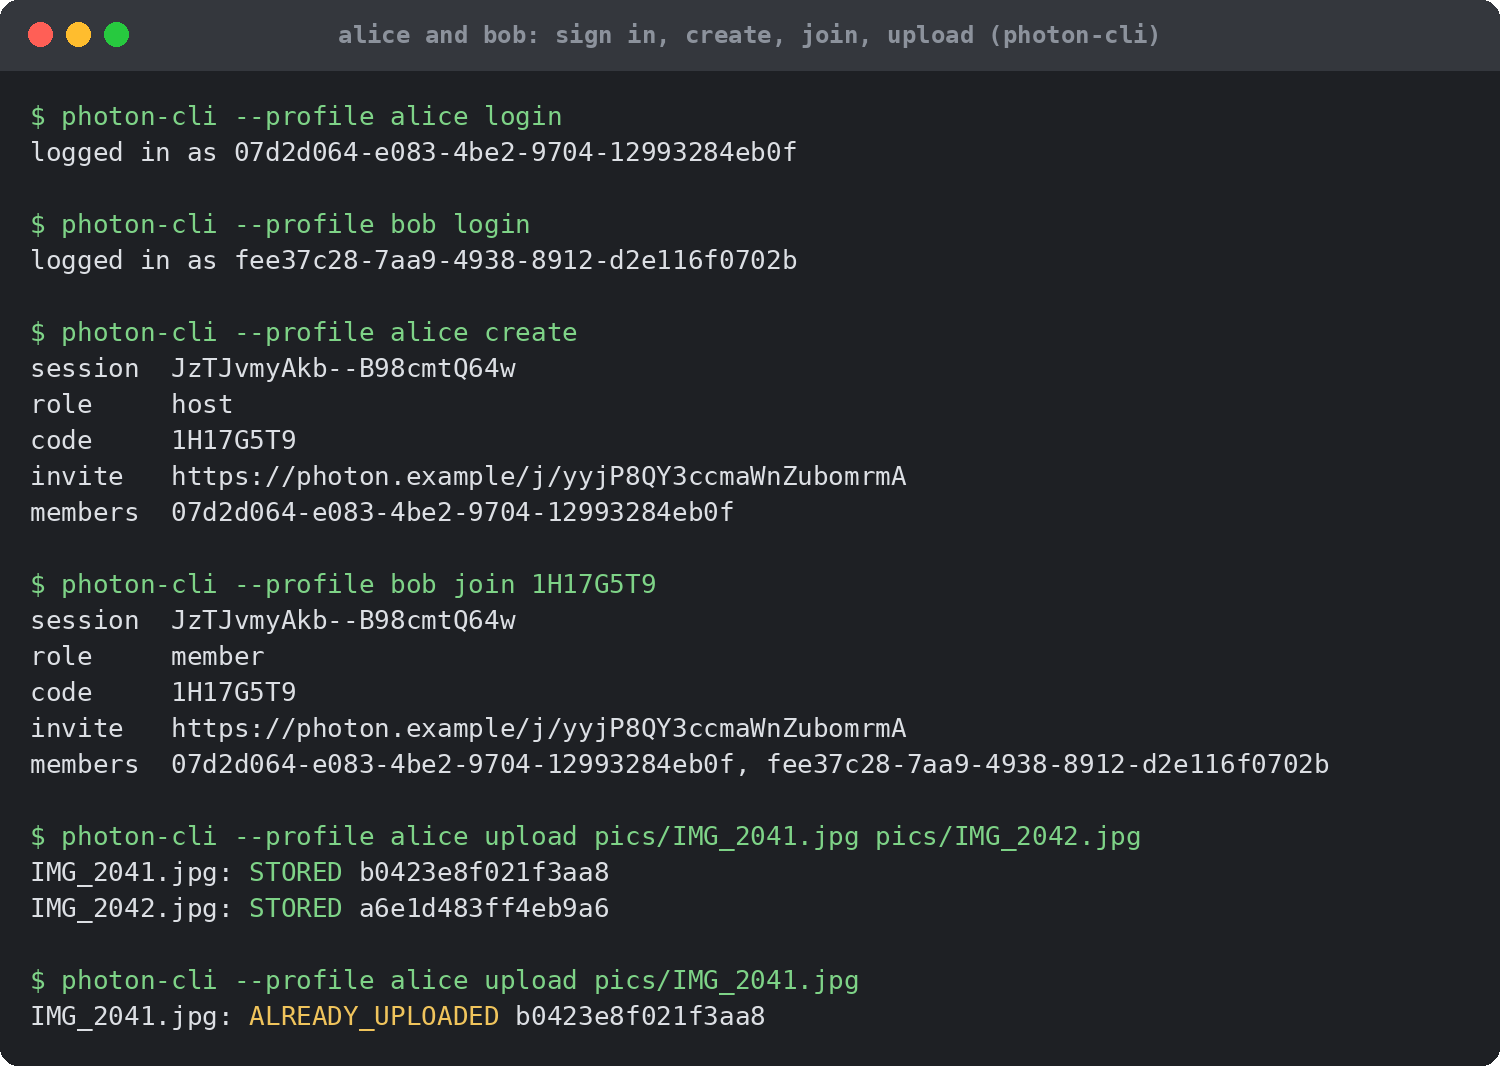
\includegraphics[width=0.78\linewidth]{screens/demo-share.png}
\caption{Alice and Bob sign in, Alice creates a session, Bob joins with the code, Alice uploads two photos, and a repeated upload is answered \texttt{ALREADY\_UPLOADED}}\label{fig:shot-share}
\end{figure}

\begin{figure}[H]
\centering
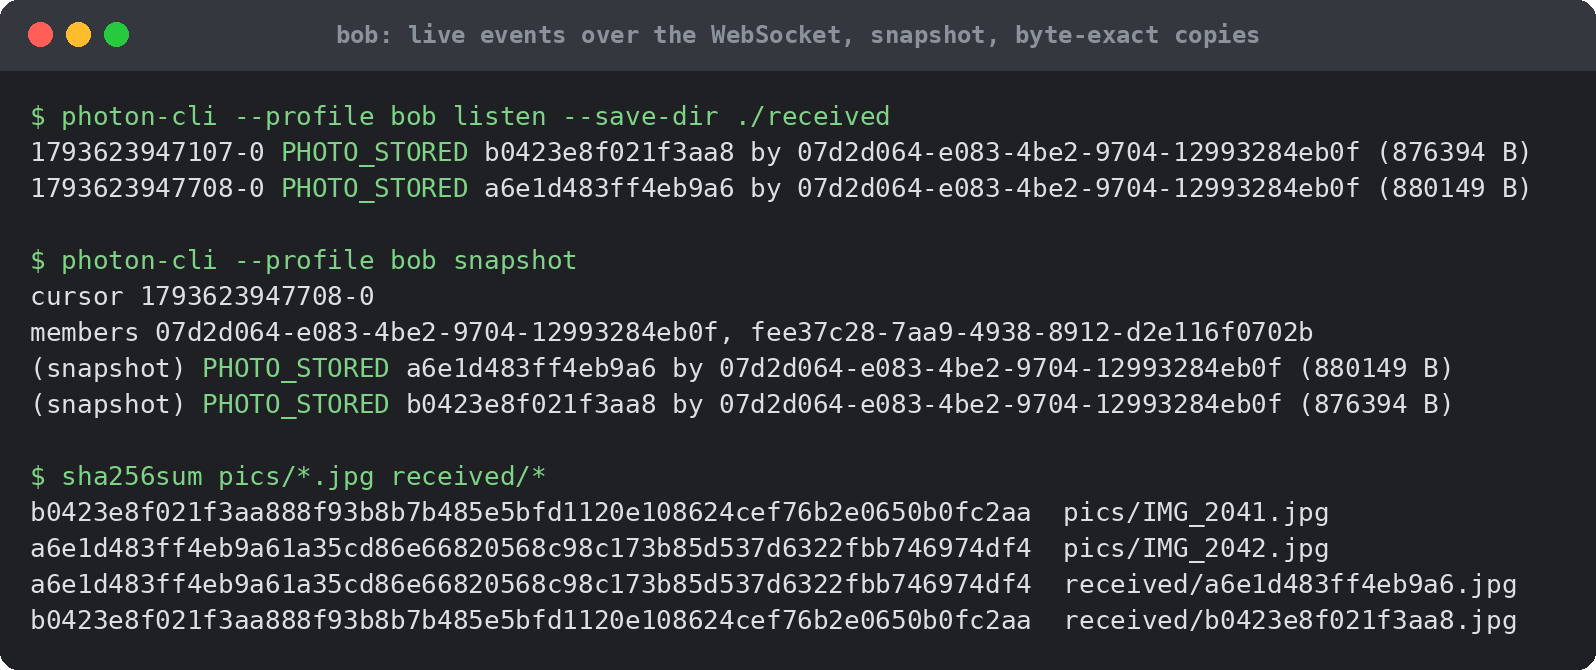
\includegraphics[width=0.86\linewidth]{screens/demo-receive.png}
\caption{Bob receives both \texttt{PHOTO\_STORED} events live over the WebSocket; the snapshot agrees; the received files are byte-identical to the originals (same SHA-256)}\label{fig:shot-receive}
\end{figure}

\begin{figure}[H]
\centering
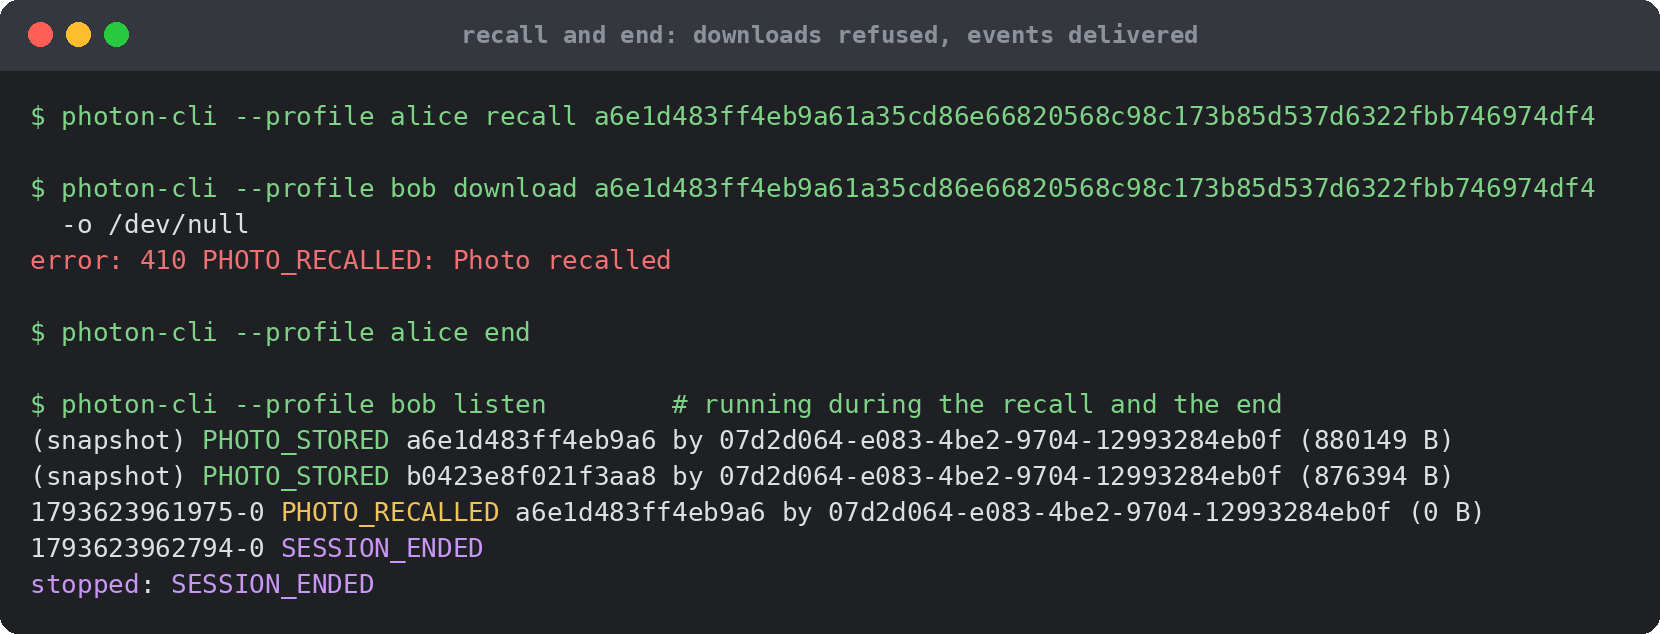
\includegraphics[width=0.86\linewidth]{screens/demo-recall.png}
\caption{Alice recalls a photo: Bob's download is refused with \texttt{410 PHOTO\_RECALLED} and his listener receives \texttt{PHOTO\_RECALLED}, then \texttt{SESSION\_ENDED} when Alice ends the session}\label{fig:shot-recall}
\end{figure}

Figure~\ref{fig:appshots} shows the Android app in a session with two members: developer sign-in, offered because the development server has no Google client configured (a); starting or joining a session (b); the session code, its QR and the members (c); and a photo from the other member, received and saved to the gallery (d).

\begin{figure}[H]
\centering
\begin{tabular}{C{3.45cm}C{3.45cm}C{3.45cm}C{3.45cm}}
\appshot{app-login.jpg}{Sign-in} & \appshot{app-home.jpg}{Start or join} & \appshot{app-session.jpg}{Live session} & \appshot{app-received.jpg}{Photo received}\\[2pt]
\small (a) Sign-in & \small (b) Start or join & \small (c) Live session & \small (d) Photo received \\
\end{tabular}
\caption{The Android app: sign-in, the home screen, a live session with two members, and the same session after a photo from the other member was received and saved}\label{fig:appshots}
\end{figure}

\subsection{Installation Guide}

\subsubsection{Run the Server and the Tests}

The server needs Python 3.12 and a C compiler (Redis 7.2 is built from source); Postgres comes from a Python wheel, so no Docker is needed for development. The Android app needs JDK 17 and the Android SDK.

\begin{pbox}{green}{Quick Start}
\begin{lstlisting}[style=code, backgroundcolor=\color{white}]
scripts/dev-deps.sh                        # builds Redis 7.2 into .devtools/
python3 -m venv .venv && .venv/bin/pip install -e ".[dev]"
.venv/bin/pytest -q                        # 155 tests
.venv/bin/photon-dev                       # API on :8080, image server on :8081
scripts/bench.sh                           # benchmarks -> tests/bench/results/latest.md
\end{lstlisting}
\end{pbox}

\subsubsection{Run on an Android Phone}

A phone reaches the laptop in one of two ways (Figure~\ref{fig:devnet}). Over USB, \texttt{adb reverse} forwards the phone's \texttt{127.0.0.1:8080} through the cable to the laptop, so the app needs no network configuration. Over Wi-Fi, the server listens on all interfaces and the app is built with the laptop's LAN address; both must be on the same subnet.

\begin{figure}[H]
\centering
\resizebox{0.7\linewidth}{!}{\fig{devnet}}
\caption{Two network paths from a test phone to the development server}\label{fig:devnet}
\end{figure}

\begin{pbox}{green}{Phone Setup}
\begin{lstlisting}[style=code, backgroundcolor=\color{white}]
scripts/phone-backend.sh                   # terminal 1: backend reachable from phones
scripts/phone-install.sh                   # terminal 2: USB: adb reverse, build, install, open
scripts/phone-install.sh --lan 10.81.x.y   # or Wi-Fi: build for the laptop's address
scripts/phone-diagnose.sh                  # if photos stop arriving
\end{lstlisting}
\end{pbox}

\subsubsection{Deploy}

\begin{pbox}{green}{Production Deployment}
\begin{lstlisting}[style=code, backgroundcolor=\color{white}]
python3 tools/gen_keys.py deploy/keys          # Ed25519 keys, one per service
scripts/make-certs.sh deploy/certs             # internal CA for Redis TLS
cp deploy/users.acl.example deploy/users.acl   # set Redis passwords
cp deploy/.env.example deploy/.env             # host names, OAuth clients
docker compose -f deploy/docker-compose.yml up -d --build
\end{lstlisting}
\end{pbox}

\subsection{Comparison with Existing Systems}

Table~\ref{tab:compare} compares PHOTON with the tools people use today to exchange event photos. The comparison is based on the publicly documented, default behaviour of each product; ``Partial'' means the feature exists only in a limited form. Figure~\ref{fig:chart-score} totals the table, counting a tick as 1 and Partial as 0.5.

\begin{table}[H]
\centering
\footnotesize\rowcolors{2}{white}{rowalt}
\begin{tabularx}{\linewidth}{YC{1.35cm}C{1.35cm}C{1.35cm}C{1.35cm}C{1.35cm}C{1.35cm}}
\headrow \hd{Feature} & \hd{PHOTON} & \hd{Google Photos} & \hd{iCloud SPL} & \hd{AirDrop} & \hd{Quick Share} & \hd{WhatsApp group}\\
Shares new camera photos with the group automatically & \cm & \pa & \cm & \xm & \xm & \xm \\
Android and iOS members in one group & \cm & \cm & \xm & \xm & \xm & \cm \\
Members need not be near each other & \cm & \cm & \cm & \xm & \xm & \cm \\
No long-lived copy on a server & \cm & \xm & \xm & \cm & \cm & \pa \\
Original quality by default & \cm & \pa & \cm & \cm & \cm & \xm \\
Thumbnail first, original later & \cm & \cm & \cm & \xm & \xm & \cm \\
Uploader can recall a shared photo & \cm & \cm & \cm & \xm & \xm & \cm \\
Time-boxed group joined by code or QR & \cm & \xm & \xm & \xm & \xm & \xm \\
Open source and self-hostable & \cm & \xm & \xm & \xm & \xm & \xm \\
\hline
\rowcolor{boxfill}\textbf{Score / 9} & \textbf{9} & \textbf{5} & \textbf{5} & \textbf{2} & \textbf{2} & \textbf{4.5} \\
\end{tabularx}
\caption{Feature comparison: PHOTON and existing photo-sharing tools}\label{tab:compare}
\end{table}

\begin{figure}[H]
\centering
\resizebox{0.68\linewidth}{!}{\fig{chart-score}}
\caption{Feature score of PHOTON and existing tools (from Table~\ref{tab:compare})}\label{fig:chart-score}
\end{figure}

The table counts only the features PHOTON was designed for. The existing tools are ahead elsewhere: WhatsApp encrypts end to end, while PHOTON's server can read a photo during its 30 minutes; Google Photos and iCloud keep long-term albums and handle video; AirDrop and Quick Share work peer to peer without any server; Apple's own library syncs in the background on iOS; and all of them are tested at a scale far beyond one machine and one phone.

\section{Conclusion}\label{sec:conclusion}

\subsection{Summary of Achievements}

PHOTON turns a group of phones into a live, shared camera roll. It solves the problem stated in Section~\ref{sec:intro} with standard protocols, used carefully:

\begin{itemize}
  \item \textbf{Verified before announced.} No member is told about a photo until the server has recomputed its SHA-256 and stored it, so content-addressed dedupe cannot be poisoned by a false claim.
  \item \textbf{Reliable over unreliable networks.} Uploads are cut into checksummed chunks sent over HTTP/3 with HTTP/2 fallback; only lost chunks are resent, and every request is idempotent, so a retry after any failure is safe.
  \item \textbf{No gaps, no duplicates.} One \texttt{XREAD} loop per socket delivers backlog and live events from the same durable stream; client-side deduplication by event id and hash turns at-least-once delivery into an exactly-once effect. Tests delivered 1{,}200 events across random reconnects, and 3{,}060 of 3{,}060 to 153 sockets.
  \item \textbf{Safe under concurrency and delay.} All state transitions are atomic Redis functions, and every cross-service report is fenced by its \texttt{upload\_id}, so a stalled client can never undo newer state.
  \item \textbf{Ephemeral by design.} Logical expiry is exact at 30 minutes, physical deletion is bounded by two independent sweepers, and there are no shareable links.
  \item \textbf{Working on a real phone.} The Android app synced photos within about 2\,s in the background, also after its process was killed and after an update; 155 server tests, 135 Android tests and 90 iOS-core tests pass.
\end{itemize}

\subsection{Limitations}

\begin{enumerate}
  \item \textbf{No end-to-end encryption.} The server can read photos during their 30 minutes. Encrypting each photo with a per-session key held only by members would remove this, at the cost of server-side thumbnails and validation.
  \item \textbf{HTTP/3 not measured on a phone.} HTTP/3 is configured at the edge and supported by the Android client, but the device tests ran against the development server over HTTP/1.1, without the edge proxy.
  \item \textbf{iOS app not compiled.} The PhotonKit core is built and tested; the SwiftUI app needs Xcode.
  \item \textbf{Single machine.} Benchmarks and the load test ran on one laptop, and the Docker deployment was written but not run on the build machine.
\end{enumerate}

\subsection{Future Work}

\begin{enumerate}
  \item \textbf{End-to-end encryption} with a session key exchanged through the join flow, and thumbnails made on the uploading phone.
  \item \textbf{Measuring HTTP/3 against HTTP/2} on real mobile links, including uploads that continue across a Wi-Fi to LTE handover through QUIC connection migration.
  \item \textbf{Peer-to-peer delivery} between phones on the same Wi-Fi network (for example with WebRTC data channels), using the server only for signalling and verification.
  \item \textbf{Object storage and Redis Cluster} for horizontal scaling; the keys already carry \texttt{\{sid\}} hash tags and the storage layout is ready for S3.
  \item \textbf{Video and Live Photos}, with resumable uploads of larger files and streaming previews.
\end{enumerate}

\subsection{Final Remarks}

The project showed that the hard part of a "simple" sharing feature is the network between the phones: lost packets, changing addresses, stalled uploads, duplicated retries and missed notifications. Each was handled with a standard mechanism from computer networks, namely QUIC, selective retransmission, idempotent requests, leases, fencing tokens and a durable event log, and each was tested both in code and on a real device.

\section{Bibliography}\label{sec:biblio}
{\renewcommand{\section}[2]{}%
\begin{thebibliography}{99}\small\setlength{\itemsep}{1pt}
\bibitem{kurose} J.~F.~Kurose and K.~W.~Ross, \emph{Computer Networking: A Top-Down Approach}, 8th ed. Pearson, 2021.
\bibitem{rfc9110} R.~Fielding, M.~Nottingham and J.~Reschke, ``HTTP Semantics,'' RFC 9110, IETF, Jun. 2022.
\bibitem{rfc9113} M.~Thomson and C.~Benfield, ``HTTP/2,'' RFC 9113, IETF, Jun. 2022.
\bibitem{rfc9000} J.~Iyengar and M.~Thomson, ``QUIC: A UDP-Based Multiplexed and Secure Transport,'' RFC 9000, IETF, May 2021.
\bibitem{rfc9114} M.~Bishop, ``HTTP/3,'' RFC 9114, IETF, Jun. 2022.
\bibitem{rfc7838} M.~Nottingham, P.~McManus and J.~Reschke, ``HTTP Alternative Services,'' RFC 7838, IETF, Apr. 2016.
\bibitem{rfc8446} E.~Rescorla, ``The Transport Layer Security (TLS) Protocol Version 1.3,'' RFC 8446, IETF, Aug. 2018.
\bibitem{rfc6455} I.~Fette and A.~Melnikov, ``The WebSocket Protocol,'' RFC 6455, IETF, Dec. 2011.
\bibitem{rfc6749} D.~Hardt, ``The OAuth 2.0 Authorization Framework,'' RFC 6749, IETF, Oct. 2012.
\bibitem{rfc7636} N.~Sakimura, J.~Bradley and N.~Agarwal, ``Proof Key for Code Exchange by OAuth Public Clients,'' RFC 7636, IETF, Sep. 2015.
\bibitem{rfc7519} M.~Jones, J.~Bradley and N.~Sakimura, ``JSON Web Token (JWT),'' RFC 7519, IETF, May 2015.
\bibitem{rfc8037} I.~Liusvaara, ``CFRG Elliptic Curve Diffie-Hellman (ECDH) and Signatures in JSON Object Signing and Encryption (JOSE),'' RFC 8037, IETF, Jan. 2017.
\bibitem{rfc7239} A.~Petersson and M.~Nilsson, ``Forwarded HTTP Extension,'' RFC 7239, IETF, Jun. 2014.
\bibitem{rfc3720} J.~Satran \emph{et al.}, ``Internet Small Computer Systems Interface (iSCSI),'' RFC 3720, IETF, Apr. 2004 (CRC32C, Appendix B.4).
\bibitem{fips180} National Institute of Standards and Technology, ``Secure Hash Standard (SHS),'' FIPS PUB 180-4, Aug. 2015.
\bibitem{kleppmann} M.~Kleppmann, \emph{Designing Data-Intensive Applications}. O'Reilly Media, 2017, ch.~8 (fencing tokens).
\bibitem{redisstreams} Redis Ltd., ``Redis Streams'' and ``Redis Functions,'' Redis documentation. Available: \url{https://redis.io/docs/latest/develop/data-types/streams/}
\bibitem{protobuf} Google, ``Protocol Buffers Language Guide (proto3).'' Available: \url{https://protobuf.dev/programming-guides/proto3/}
\bibitem{fcm} Google, ``Firebase Cloud Messaging.'' Available: \url{https://firebase.google.com/docs/cloud-messaging}
\bibitem{apns} Apple Inc., ``Sending notification requests to APNs.'' Available: \url{https://developer.apple.com/documentation/usernotifications}
\bibitem{adb} Android Developers, ``Android Debug Bridge (adb).'' Available: \url{https://developer.android.com/tools/adb}
\bibitem{workmanager} Android Developers, ``Schedule tasks with WorkManager'' and ``Foreground services.'' Available: \url{https://developer.android.com/develop/background-work}
\bibitem{caddy} Caddy Web Server documentation, ``Global options: protocols.'' Available: \url{https://caddyserver.com/docs/caddyfile/options}
\end{thebibliography}}


\end{document}
